\ifdefined\standalone
\documentclass[12pt]{article}
\usepackage{graphicx}
\usepackage{float}
\usepackage[a4paper, margin=1in]{geometry}
\usepackage[utf8]{inputenc}
\usepackage{textcomp}
\usepackage{amsmath}
\usepackage{booktabs}
\usepackage[hidelinks]{hyperref}
\begin{document}
\fi

\section{3-D Heat Diffusion in a Steel I-Beam}

This case is intended to verify the Gpyro code under three-dimensional heat diffusion conditions involving a complex I-beam geometry. 
A steel I-beam is considered, with an overall square cross-section of $0.4$~m on each side. The flanges are $6$~cm thick, while the web has a thickness of $4$~cm, as shown in Figure~\ref{fig:ibeam_geom}.

The spatial grid resolution used in both the Gpyro and FDS simulations is $\Delta x =\Delta y =\Delta z = 1$~cm. The thermal properties of the steel are assumed to be constant, with a thermal conductivity $k = 45$~W\,m$^{-1}$\,K$^{-1}$, a density $\rho = 7850$~kg\,m$^{-3}$, and a specific heat capacity $c = 0.60$~kJ\,kg$^{-1}$\,K$^{-1}$.

All boundary conditions are adiabatic, except for a heated patch located on the front half of the bottom flange, which is maintained at a constant temperature of $800\,^{\circ}$C. The initial temperature of the steel is set to $20\,^{\circ}$C. The simulation is run for a total duration of $3600$~s.

Temperatures are monitored at six locations within the beam, as indicated in Figure~\ref{fig:ibeam_geom}. The temporal evolution of the temperature at these points is presented in Figure~\ref{fig:ibeam_points}. In addition, temperature profiles are extracted along the $x$ and $z$ directions at different times and are shown in Figure~\ref{fig:ibeam_profile}.


\begin{figure}[H]
\centering
  \begin{minipage}{0.33\linewidth}
  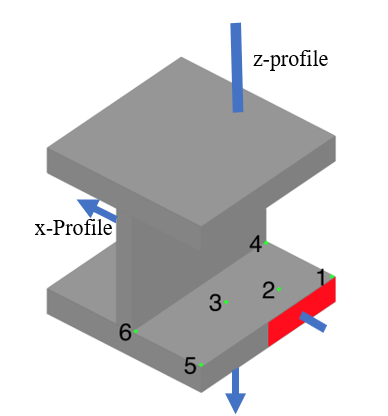
\includegraphics[width=\textwidth]{I_beam_schematic.png}
  \caption{I-beam geometry ~\cite{FDS_Verif}}
  \label{fig:ibeam_geom}
  \end{minipage}
   \hfill
  \begin{minipage}{0.65\linewidth}
  \includegraphics[width=\textwidth]{I_beam_point_T.png}
  \caption{Time evolution of Temperature at the measurement points.}
  \label{fig:ibeam_points}
  \end{minipage}
\end{figure}

\begin{figure}[H]
\centering
\includegraphics[width=0.45\textwidth]{I_beam_y_profile.png}
\hfill
\includegraphics[width=0.45\textwidth]{I_beam_z_profile.png}
\caption{Temperature profiles along the $x$ direction (left) and along the $z$ direction (right) at different times.}
\label{fig:ibeam_profile}
\end{figure}

\ifdefined\standalone
\end{document}
\fi
